\chapter{Extensions}\label{extensions}
In the same spirit as~\cite{nips-dqn} with experience replay and frameskip, we try a couple of extensions to the basic algorithm of DQN.

\section{Dropout}
Training a basic RAM-only network leads to high variance of the results (see the figures \labelcref{fig:breakout-plain,fig:seaquest-plain,fig:bowling-plain}) over epochs. This can be a sign of overfitting. To tackle this problem we applied dropout~\cite{dropout}, a standard regularization technique for neural networks.

Dropout is a simple, yet effective regularization method. It consists of ``turning off'' with probability~$p$ each neuron in training, i.e. setting the output of the neuron to~$0$, regardless of its input. In backpropagation, the parameters of switched off nodes are not updated. Then, during testing, all neurons are set to ``on''---they work as in the course of normal forward pass, with the exception that each neuron's output is multiplied by~$p$ to make up for the skewed training.

The intuition behind the dropout method is that it forces each node to learn in absence of other nodes. The work~\cite{dropout-variance} shows an experimental evidence that the dropout method indeed reduces the variance of the learning process.

We have enabled dropout with probability of turning off a neuron~$p = \frac{1}{2}$. This applies to all nodes, except output ones. We implemented dropout for both RAM-only networks: \texttt{just\_ram} and~\texttt{big\_ram}. The progress of training for Seaquest is show in figure \ref{fig:seaquest-dropout} and the best epoch results are presented in the table \ref{table:results-dropout}. This method offers an improvement for the \texttt{big\_ram} network for Seaquest, leading to the best results for this game in this paper.

\begin{figure}[h]
\centering
\begin{tikzpicture}[scale=1]
\begin{axis}[
   xlabel={Training epoch},
   ylabel={Average score per episode},
   xmin=0,xmax=101,
   x=0.12cm,
   grid=major,
   mark options={solid, scale=0.35},
   legend entries={\texttt{just\_ram}, \texttt{big\_ram}},
   legend style={legend pos=north west},
]
\addplot[mark=*, color=blue, line width=0.25pt] table {experiments/seaquest_just_dropout.txt};
\addplot[mark=*, color=red, line width=0.25pt] table {experiments/seaquest_big_dropout.txt};
\addplot[mark=*, color=blue, only marks, mark size=5] table {
x	y
74	1246.66666667
};
\addplot[mark=*, color=red, only marks, mark size=5] table {
x	y
97	2805.0
};
\end{axis}
\end{tikzpicture}
\caption{Training results for Seaquest with dropout~$p=0.5$ for models \texttt{just\_ram}, \texttt{big\_ram}. The figure suggests that indeed dropout reduces the variance of the learning process.}
\label{fig:seaquest-dropout}
\end{figure}

\begin{table}[h]
\centering
\begin{tabularx}{0.8\textwidth}{ X c c c }
  \toprule
  & Breakout & Seaquest & Bowling \\
  \midrule
  \texttt{just\_ram with dropout} best & $130.5$  & $1246.67$ & $54.75$ \\
  \texttt{big\_ram with dropout} best & $122.25$ & \textbf{2805} & $58.25$\\
  \bottomrule
\end{tabularx}
\caption{Summary of test results for training which involves dropout with the parameter $p=0.5$.}
\label{table:results-dropout}
\end{table}

\section{Learning rate}
The high variance in training, as illustrated by figures~\cref{fig:breakout-plain,fig:seaquest-plain,fig:bowling-plain}, could be caused by setting a too high learning rate. It may come from ``stepping over'' optimal values when taking too big steps in the parameter space by the RMSProp algorithm. If it was the case, decreasing the step size should lead to slower learning combined with higher precision of finding minima of the loss function and better results.

We performed the experiments with reduction of learning rate from~$0.0002$ to~$0.0001$. The results of them can be found in table~\ref{table:rate}. Comparing to the training without dropout, scores improved only in the case of Breakout and the \texttt{just\_ram} network, but not by a big margin.

\begin{table}[h]
\centering
\begin{tabularx}{0.7\textwidth}{ X c c c }
  \toprule
  &\ Breakout\ &\ Seaquest & Bowling \\
  \midrule
  \texttt{just\_ram} best & $137.67$ & $1233.33$ & $51.5$ \\
  \texttt{big\_ram} best  & $112.14$ & $2675$ & $59.25$ \\
  \bottomrule
\end{tabularx}
\caption{Summary of test results for modified learning rate.}
\label{table:rate}
\end{table}
\section{Frameskip}\label{our-frameskip}
In the benchmark agent \texttt{nips}, authors use the frameskip (see section~\ref{frameskip} for definition of frameskip) value of~$4$ and pass for training \emph{all} $4$~frames before the action to handle ``blinking'' behavior of Atari machine, i.e. showing some objects only every couple of frames.
In the case of learning from memory there is no loss of information when previous RAM~states are ignored. Hence in our models we only pass to the network the RAM~state corresponding to the last frame before a given action. We made some limited experiments passing all previous \texttt{frameskip} RAM~states to the network, but the results were worse than when passing only the last one. We still used frameskip of~$4$ in the basic experiments.

The work~\cite{frameskip} suggests that choosing the right frameskip has a big influence on the performance of a model (see also~\cite{microsoft-frameskip}). We decided to try two bigger values of frameskip: $8$ and~$30$, corresponding to deciding on actions~$5$ and~$2$ times a second.

The figure~\ref{fig:seaquest-frameskip} and table~\ref{table:results-frameskip} show a significant improvement of the \texttt{just\_ram} model in Seaquest, as well as the \texttt{big\_ram} model for Bowling. Quite surprisingly, the variance of the results appeared to be much lower with higher frameskip for all tested models.

\begin{figure}[h]
\centering
\begin{tikzpicture}[scale=1]
\begin{axis}[
   xlabel={Training epoch},
   ylabel={Average score per episode},
   xmin=0,xmax=101,
   x=0.12cm,
   grid=major,
   mark options={solid, scale=0.35},
   legend entries={$\texttt{frameskip} = 8$, $\texttt{frameskip} = 30$},
   legend style={legend pos=north west},
]
\addplot[mark=*, color=blue, line width=0.25pt] table {experiments/seaquest_just_fs8.txt};
\addplot[mark=*, color=red, line width=0.25pt] table {experiments/seaquest_just_fs30.txt};
\addplot[mark=*, color=blue, only marks, mark size=5] table {
x	y
85	2064.44444444
};
\addplot[mark=*, color=red, only marks, mark size=5] table {
x	y
100	2093.24324324
};
\end{axis}
\end{tikzpicture}
\caption{Training results for Seaquest with 
$\texttt{frameskip} = 8$ and  $\texttt{frameskip} = 30$ for the model \texttt{just\_ram}.}
\label{fig:seaquest-frameskip}
\end{figure}

\begin{table}[h]
\centering
\begin{tabularx}{0.9\textwidth}{ X c c c }
  \toprule
   &\ Breakout\ &\ Seaquest\ & Bowling \\
  \midrule
  \texttt{just\_ram} with \texttt{frameskip} $8$ best & $82.87$  & $2064.44$ & $54.56$\\
  \texttt{just\_ram} with \texttt{frameskip} $30$ best & -  & $2093.24$ & $54.36$\\
  \texttt{big\_ram} with \texttt{frameskip} $8$ best & $102.64$ & $2284.44$ & $\textbf{70.78}$ \\
  \texttt{big\_ram} with \texttt{frameskip} $30$ best & - & $2043.68$ & $61.9$\\
  \bottomrule
\end{tabularx}
\caption{Table summarizing test results for training which involves higher \texttt{frameskip} value. For Breakout $\texttt{frameskip} 
=30$ does not seem to be a suitable choice.}
\label{table:results-frameskip}
\end{table}

As noticed in~\cite{frameskip}, in the case of Breakout high frameskips, such as~$30$ lead to a disastrous performance, thus we tested only frameskip~$8$ and for it we received slightly weaker results than with a baseline frameskip~$4$.

\section{Joining RAM and screen}\label{screen-ram-networks}

An interesting question regarding learning agents playing Atari games is whether it is possible to combine information from the screen and RAM and create an agent that would successfully use both sources of information. This subsection makes first steps to towards answering this question.

We consider two mixed network architectures. The first one is \texttt{mixed\_ram}, where we just concatenate output of the last hidden layer of the convolutional network with the RAM input and then apply a linear transformation with no non-linearity. It is worth to remind that the RAM input, as well as screen are scaled down to be in range~$[0, 1]$; with no normalization a disastrous performance was observed.

%%%%%%%%%%%%%%%%%%%%%%%%%%%%%%%%%%%%%%%%%%%%%%%%%%%%%%%%%
\RestyleAlgo{ruled}
\begin{algorithm}[H]
\SetAlgoRefName{3}
\caption{\texttt{mixed\_ram} (numActions)}

\SetAlgoVlined
\DontPrintSemicolon
% \LinesNumbered

\KwIn{RAM, screen} 
\KwOut{A vector of length numActions}
\vspace{0.05cm}

conv1 $\leftarrow$ Conv2DLayer(screen, rectify)\;
conv2 $\leftarrow$ Conv2DLayer(conv1, rectify)\;
hidden $\leftarrow$ DenseLayer(conv2, $256$, rectify)\;
concat $\leftarrow$ ConcatLayer(hidden, RAM)\;
output $\leftarrow$ DenseLayer(concat, numActions, no activation)\;

\Return{{\upshape output}}
\end{algorithm}

%%%%%%%%%%%%%%%%%%%%%%%%%%%%%%%%%%%%%%%%%%%%%%%%%%%%%%%%%
The other architecture is a deeper version of \texttt{mixed\_ram}. We use more dense layers which are applied in a more sophisticated way as described below.

%%%%%%%%%%%%%%%%%%%%%%%%%%%%%%%%%%%%%%%%%%%%%%%%%%%%%%%%%
\RestyleAlgo{ruled}
\begin{algorithm}[H]
\SetAlgoRefName{4}
\caption{\texttt{big\_mixed\_ram} (numActions)}

\SetAlgoVlined
\DontPrintSemicolon
% \LinesNumbered

\KwIn{RAM, screen} 
\KwOut{A vector of length numActions}
\vspace{0.05cm}

conv1 $\leftarrow$ Conv2DLayer(screen, rectify)\;
conv2 $\leftarrow$ Conv2DLayer(conv1, rectify)\;
hidden1 $\leftarrow$ DenseLayer(conv2, $256$, rectify)\;
hidden2 $\leftarrow$ DenseLayer(RAM, $128$, rectify)\;
hidden3 $\leftarrow$ DenseLayer(hidden2, $128$, rectify)\;
concat $\leftarrow$ ConcatLayer(hidden1, hidden3)\;
hidden4 $\leftarrow$ DenseLayer(concat, $256$, rectify)\;
output $\leftarrow$ DenseLayer(hidden4, numActions, no activation)\;

\Return{{\upshape output}}
\end{algorithm}
\SetAlgorithmName{Algorithm}{List of Algorithms}
%%%%%%%%%%%%%%%%%%%%%%%%%%%%%%%%%%%%%%%%%%%%%%%%%%%%%%%%%

The results, which are presented in table~\ref{table:mixed} are reasonable, but not impressive. In particular, we did not see any improvement over the benchmark \texttt{nips} agent, which is embedded into both mixed architectures. This suggests that in \texttt{mixed\_ram} and \texttt{big\_mixed\_ram} models the additional information about the RAM state is not used in a productive way.

\begin{table}[h]
\centering
\begin{tabularx}{0.7\textwidth}{ X c c c }
  \toprule
  &\ Breakout\ &\ Seaquest\ & Bowling \\
  \midrule
  \texttt{mixed\_ram} best & $143.67$ & $488.57$ & $39.5$\\
  \texttt{big\_mixed\_ram} best  & $67.56$ & $1700$ & $45.5$\\
  \bottomrule
\end{tabularx}
\caption{Table summarizing test results for methods combining information from the screen and from the memory.}
\label{table:mixed}
\end{table}

\section{RNN}
\optional{If we tried RNN tell what happened}

\section{RAM visualization}
To better understand how the agents work, we visualized in figure~\ref{fig:ram-vis} the first layers of the network \texttt{big\_ram} in Breakout and Seaquest. 

\begin{figure}[!h]
\centering
\subfigure[\texttt{big\_ram} in Breakout]{
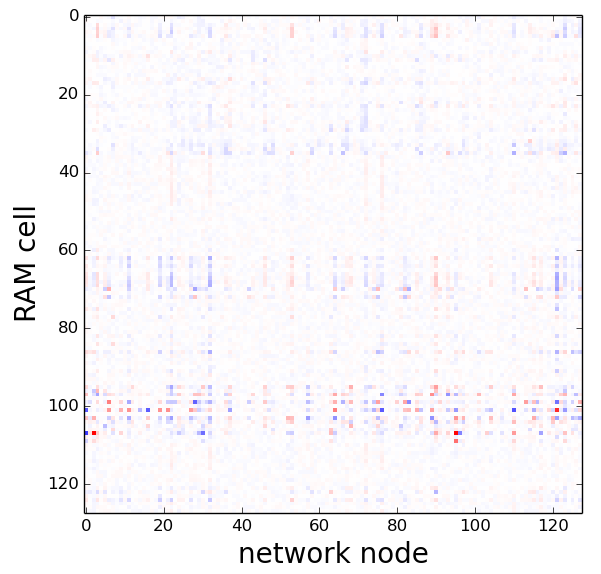
\includegraphics[scale=0.45]{images/axis_breakout_plot_cut.png}
}
\hspace{15pt}
\subfigure[\texttt{big\_ram} in Seaquest]{
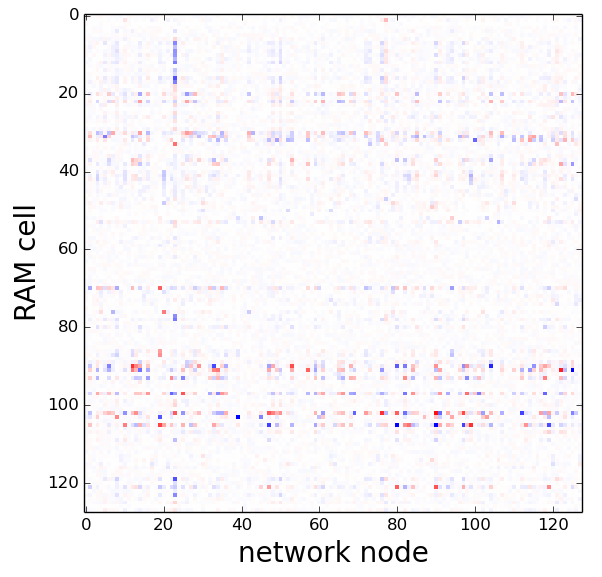
\includegraphics[scale=0.449]{images/axis_seaquest_plot_cut.png}
}
\caption{Visualization of the parameters of the first layer of the trained Q-networks.}
\label{fig:ram-vis}
\end{figure}

Each column corresponds to one of $128$~nodes in the first layer of the trained network and each row corresponds to one of $128$~memory~cells. The color of a grid cell describes whether the high value in a given RAM~cell negatively (blue) or positively (red) influences the activation level for a given neuron.

Figure~\ref{fig:ram-vis} suggests that the RAM~cells with numbers $95$--$105$ are important for gameplay---the activation of many neurons of the \texttt{big\_ram} network depend on the state of these cells.
